% version 1

\documentclass[10point]{article}

% prelude

\usepackage{fancyvrb}
\usepackage{graphicx}
\usepackage[pdftex, backref, colorlinks, bookmarksnumbered=true]{hyperref}

\DefineVerbatimEnvironment{code}{Verbatim}{}

\newcommand{\highlight}[1]{\colorbox{yellow}{#1}}
\newcommand{\highlighttt}[1]{\highlight{{\tt#1}}}

\long\def\ignore#1{}

\begin{document}

\title{Visuals Report}
\author{Callum McColl\\
	    Andrew Paroz}
		
\maketitle

\begin{abstract}
We did stuff. And more stuff, then stuff happened.
\end{abstract}

\tableofcontents

\listoffigures

\section{Introduction}
The goal of this project was to create a program that could compile, execute and displayed a C program. It could then be used to go step-by-step through a C program in order to show how the memory and registers are effected by each line of C code. In order to learn functional programming and Mash as a template, this program was created using Haskell. The project could be divided into 5 separate sections, the C parser, the assembly parser, C to assembly code generation, the emulator and the GUI. These were then allocated to three groups, one group would create the C Parser, another the Assembly Parser and Symbol Table, and the last group the Emulator and GUI. The Code generation which converts a C Parse tree to an Assembly Parse tree was not assigned to any group. A diagram of this can be see in Figure \ref{fig:ProjectDiagram}.

\begin{figure}
{\centering

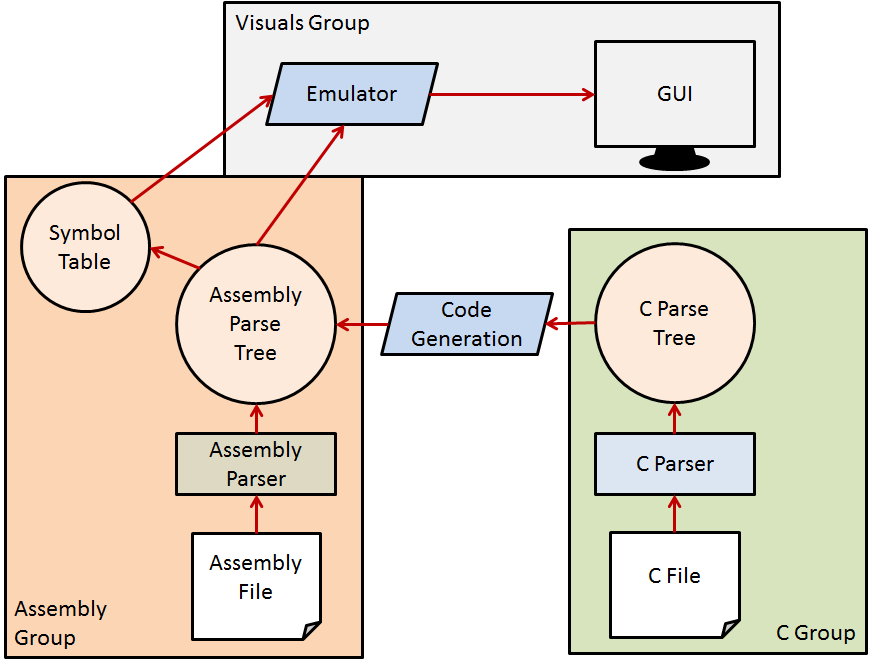
\includegraphics[width=300px]{ProjectDiagram}
\label{fig:ProjectDiagram}
\caption{Project diagram showing all the main parts and group allocations.}
}
\end{figure}

The program that this project created is to be used as a learning tool to help teach C programming. C is a difficult language when starting as there are multiple ways to do the same thing in the language, but some ways are more 'right' than others. The compilers can also be very lenient and compile and run code that is not correct, leading to problems where code ends up running differently on different systems. By having a program that can go step-by-step through a C program, it will be much easier to show why errors are, and explain to students why a program is acting in that way.

Obviously the C language is very vast, so only a small subset was chosen to a implemented for this project. All variables are either an Int or a pointer, there are no structs and everything must be contained within a single file. Due to the complexity of converting a C parse tree to an assembly parse tree, that part of the project was dropped

\section{Process and Design}
Describe process / design

\section{Design Details}
Details about the design.

\section{Implementation}
\subsection{Environment}
\input{../Environment.lhs}

\subsection{Emulation}
\input{../Emulation.lhs}

\subsection{GUI}
- Callum fill this.

\section{Results, evidence of what works}
Screenshots of the GUI and output of printing an environment I guess.

\section{Conclusion}

\subsection{Callum McColl's Reflection}

\subsection{Andrew Paroz's Reflection}


\end{document}



